\chapter{Applications}
\label{ch:applications}


\section{Areas of application}
\label{sect:app_areas}

	\subsection{Social networks}
	\label{ssect:social_networks}
	
	Network recommendations
	
	The recommender cascade paper...
	
	* in the present paper, we are able to observe the cascades but not the underlying social network
	* In our work we need to efficiently enumerate and count cascade subgraphs
	* most of the prior work in this area is focused on graphs that are richly
	labeled and undirected, often motivated by applications to chemical compound
	and bioinformatics datasets
	* subgraphs based purely on their structures
	* The first recipient to purchase the item received a discount, and the sender received a referral credit with monetary value. A person could make recommendations on a product only after purchasing it. Since each sender had an incentive for making effective referrals, it is natural to hypothesize that this dataset is a good source of cascades.
	* Recommendation network is not the same as the underlying social network structure; actually, only the recommendation network was considered in their analysis of cascades.
	* recommendation subgraphs of the different products (DVDs, books, etc.)
	* all networks are very sparsely linked
	* At the end of the two-year period, the largest connected component contained fewer than 2.5% of the nodes
	* Observe that for DVDs 9% of purchases are associated with a recommendation, for books 3%, music 1.5% and video less than 1%.
	* One might imagine cascades to be trees or near-trees. In fact, we find that recommendations create essentially arbitrary graphs: there can be multiple recommendations on the same product or multiple product recommendations between the same pair of nodes; there are multiple purchases of the same product by the same individual (this is natural given that many items are purchased as gifts); and one also finds many cycles.
	- Delete late recommendations
	- Delete all nodes that didn't purchase the product
	* Cascades form graphs, and it's necessary to figure out which cascades are similar to one another -> graph isomorphism problem
	- Why is similarity important? To figure out how many **types** of cascades exist.
	- No *polynomial-time* algorithm is known for the graph isomorphism problem
	- Heuristic approximation via a graph **signature**
	- nr. of nodes
	- nr. of edges
	- sorted in- and out-degrees (degree distribution?)
	- graphs less than 9 nodes: exact matching
	- graphs < 500 nodes: also include the singular values of the adjacency matrix (via singular value decomposition)
	- a small minority of cascades are larger than 9 nodes
	* Results:
	- For books the largest cascade has 95 nodes and 231 edges. For DVDs the largest cascade is eight times larger (n = 791, e = 5544). The cascades involving music or videos are much smaller; the largest cascades are n = 13, e = 56 and n = 37, e = 169 respectively
	- For DVDs, the log fit function of cascade size to count is similar to books and music for smaller sized cascades, and exhibit unique behavior for larger cascades, which in this experiments were only found for the DVD category.
	- the number of purchases decaying as a function of rank faster than the number of recommendations does
	- **Make table**: For books we identified 122,657 cascades, of which 959 are topologically different. There are 213 cascades that occur at least ten times. For DVDs we identified 289,055 cascades, 87,614 are topologically different, and 3,015 cascades occur at least ten times. For music we identified 13,330 cascades, 158 were topologically different, and only 23 cascades occurred at least ten times. Videos were the least rich, with 1,928 subgraphs containing 109 unique patterns, and only 12 subgraphs occurring at least ten times.
	- Splits are more frequent than collisions
	* Conclusion:
	- Recommendations -> Complex social behavior
	- NOT ONLY STATISTICALLY WITH GENERAL NETWORK PROPERTIES
	- A concluding, general observation is that the frequency of cascade subgraphs does not simply decrease monotonically in the number of nodes and edges; for example, G5 is more frequent than either of its subgraphs G2 and G4 in DVDs and videos (and more frequent than G4 in books and music). Thus, frequency appears to reflect properties of the underlying social network (the clustering of people who know each other), as well as properties of the ways in which recommendations typically get made (e.g. splits are more common than collisions)
	
	The local sphere recommender
	
	\subsection{Communication networks}
	\label{ssect:app_communication_networks}
	
	\subsection{Transportation networks (Logistics)}
	\label{ssect:app_transportation_networks}
	
	\subsection{Graph based image processing}
	\label{ssect:app_graph_img_proc}
	
	\begin{figure}[ht]
		\label{fig_graph_based_img_classification}
		\begin{center}
			
\includegraphics[width=1\textwidth]{figures/graph_img_class}
			\caption{Graph based image classification example}
		\end{center}
		\small
		1) a laser scan image of a nevus is oversegmented and 2) a graph extracted by interpreting region centroids as nodes and region adjacency as edges. 3) A belief propagation algorithm is applied to the resulting graph yielding 2) a converged state representing the nevus classification as benign or malignant.
	\end{figure}
	
	\subsection{Graph based NLP}
	\label{ssect:app_graph_nlp}
	
	\subsection{Biomedical applications (protein networks etc.)}
	\label{ssect:app_biomed}
	
	\subsection{Anonymization}
	\label{ssect:app_snonymization}
	
	\begin{figure}[ht]
		\label{fig_graph_based_img_classification}
		\begin{center}
			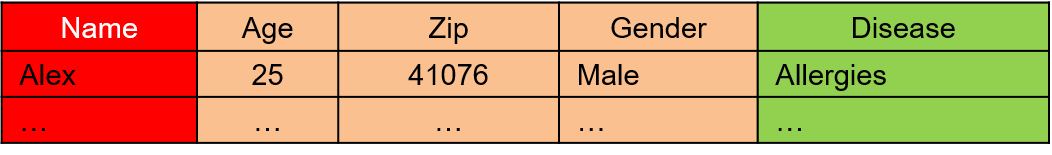
\includegraphics[width=0.9\textwidth]{figures/anonym/3typesofdata}
			\caption{The three types of data considered in (k-)anonymization}
		\end{center}
	\end{figure}
	
	
	\begin{figure}[H]
		\centering
		\begin{minipage}[b]{0.5\textwidth}
			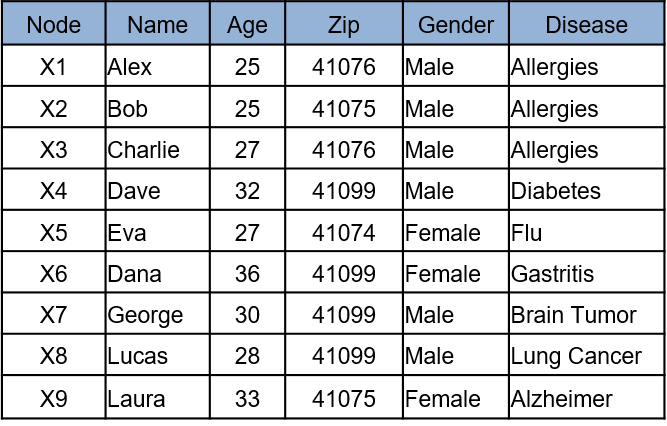
\includegraphics[width=\textwidth]{figures/anonym/k_anon_input}
		\end{minipage}
		\hfill
		\begin{minipage}[b]{0.418\textwidth}
			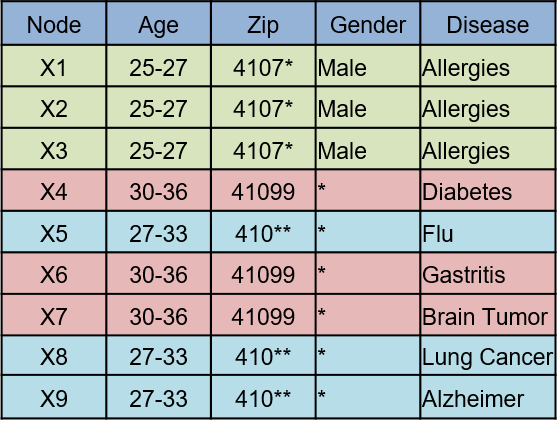
\includegraphics[width=\textwidth]{figures/anonym/k_anon_output}
		\end{minipage}
		\caption{Tabular anonymization: input table and anonymization result}
	\end{figure}	
	
	
	\subsection{Fraud detection}
	\label{ssect:fraud_detection}

	Polo chau's BP in MRF for spam classification work...

\section{Application specific requirements}
\label{section:app_requirements}

	\subsection{Data Structures}
	\label{ssect:data_gathering}
	
	\subsection{Data Cleaning}
	\label{ssect:data_cleaning}
	
	\subsection{Preprocessing}
	\label{ssect:preprocessing}
	
	Graph generation (ER model...)
	
	\subsection{Feature Selection}
	\label{ssect:feature_selection}
	
	\subsection{Data Mining}
	\label{ssect:data_mining}
	
	\subsection{Postprocessing}
	\label{ssect:postprocessing}
	
	\subsection{Visualization}
	\label{ssect:visualization}
	
	\subsection{Interaction / user feedback (iML)}
	\label{ssect:interaction}
	